%%%%%%%%%%%%%%%%%%%%%%%%%%%%%%%%%%%%%%%%%%%%%%%%%%%%%%%%%%%%%%%%%%%%%%%%%%%%%%%%
% Template for USENIX papers.
%
% History:
%
% - TEMPLATE for Usenix papers, specifically to meet requirements of
%   USENIX '05. originally a template for producing IEEE-format
%   articles using LaTeX. written by Matthew Ward, CS Department,
%   Worcester Polytechnic Institute. adapted by David Beazley for his
%   excellent SWIG paper in Proceedings, Tcl 96. turned into a
%   smartass generic template by De Clarke, with thanks to both the
%   above pioneers. Use at your own risk. Complaints to /dev/null.
%   Make it two column with no page numbering, default is 10 point.
%
% - Munged by Fred Douglis <douglis@research.att.com> 10/97 to
%   separate the .sty file from the LaTeX source template, so that
%   people can more easily include the .sty file into an existing
%   document. Also changed to more closely follow the style guidelines
%   as represented by the Word sample file.
%
% - Note that since 2010, USENIX does not require endnotes. If you
%   want foot of page notes, don't include the endnotes package in the
%   usepackage command, below.
% - This version uses the latex2e styles, not the very ancient 2.09
%   stuff.
%
% - Updated July 2018: Text block size changed from 6.5" to 7"
%
% - Updated Dec 2018 for ATC'19:
%
%   * Revised text to pass HotCRP's auto-formatting check, with
%     hotcrp.settings.submission_form.body_font_size=10pt, and
%     hotcrp.settings.submission_form.line_height=12pt
%
%   * Switched from \endnote-s to \footnote-s to match Usenix's policy.
%
%   * \section* => \begin{abstract} ... \end{abstract}
%
%   * Make template self-contained in terms of bibtex entires, to allow
%     this file to be compiled. (And changing refs style to 'plain'.)
%
%   * Make template self-contained in terms of figures, to
%     allow this file to be compiled. 
%
%   * Added packages for hyperref, embedding fonts, and improving
%     appearance.
%   
%   * Removed outdated text.
%
%%%%%%%%%%%%%%%%%%%%%%%%%%%%%%%%%%%%%%%%%%%%%%%%%%%%%%%%%%%%%%%%%%%%%%%%%%%%%%%%

\documentclass[letterpaper,twocolumn,10pt]{article}
\usepackage{usenix2019_v3}

% to be able to draw some self-contained figs
\usepackage{tikz}
\usepackage{amsmath}

% inlined bib file
\usepackage{filecontents}

%-------------------------------------------------------------------------------
\begin{filecontents}{\jobname.bib}
%-------------------------------------------------------------------------------
@Book{arpachiDusseau18:osbook,
  author =       {Arpaci-Dusseau, Remzi H. and Arpaci-Dusseau Andrea C.},
  title =        {Operating Systems: Three Easy Pieces},
  publisher =    {Arpaci-Dusseau Books, LLC},
  year =         2015,
  edition =      {1.00},
  note =         {\url{http://pages.cs.wisc.edu/~remzi/OSTEP/}}
}
@InProceedings{waldspurger02,
  author =       {Waldspurger, Carl A.},
  title =        {Memory resource management in {VMware ESX} server},
  booktitle =    {USENIX Symposium on Operating System Design and
                  Implementation (OSDI)},
  year =         2002,
  pages =        {181--194},
  note =         {\url{https://www.usenix.org/legacy/event/osdi02/tech/waldspurger/waldspurger.pdf}}}
\end{filecontents}

%-------------------------------------------------------------------------------
\begin{document}
%-------------------------------------------------------------------------------

%don't want date printed
\date{}

% make title bold and 14 pt font (Latex default is non-bold, 16 pt)
\title{\Large \bf Indicus: Unchaining Byzantine Databases\\
 }

%for single author (just remove % characters)
\author{
{\rm Your N.\ Here}\\
Your Institution
\and
{\rm Second Name}\\
Second Institution
% copy the following lines to add more authors
% \and
% {\rm Name}\\
%Name Institution
} % end author

\maketitle

%-------------------------------------------------------------------------------
\begin{abstract}
%-------------------------------------------------------------------------------
Your abstract text goes here. Just a few facts. Whet our appetites.
Not more than 200 words, if possible, and preferably closer to 150.
\end{abstract}


%-------------------------------------------------------------------------------
\section{Introduction}
%-------------------------------------------------------------------------------



There is an increasing tension between the desire to share data online, and the security concerns it entails.
This paper asks the question: how can we enable \textit{mutually distrustful parties} to consistently and reliably
share data, while minimizing centralization?

The ability to share data online offers exciting opportunities.
\iffalse %% the medical record example is for privacy, more related to Obladi, but not BFT Tapir
In the medical domain, for
instance, cloud-based solutions for managing health record offer doctors increased fault-tolerance at lower
cost, and offer patient an easier path to share their medical
history with their entire treatment teams, even when on the road. Opportunities abound in other areas too.
\fi
In banking, systems like SWIFT enable financial institutions to quickly and accurately receive information
such as money transfer instructions; and in manufacturing, online data sharing can improve accountability
and auditing amongst the globally distributed supply chain.

Increased data sharing, however, raises questions of how to \textit{decentralize trust}.
\iffalse
Even when medical records are
encrypted or anonymized, cloud providers or dishonest applications may be able to acquire
sensitive information: for example, tracking the charts accessed by an oncologist can reveal not only whether
a patient has cancer, but also, depending on the frequency of accesses (e.g., the frequency of chemotherapy
appointments), indicate the cancers type and severity.
\fi
Banking institutions must currently place their trust
in the centralized SWIFT’s network to issue payment orders. Sometimes there is even no identifiable source of
trust. Consider the supply chain for the latest iPhone: it spans three continents, and hundreds of different
contractors~(https://www.apple.com/supplier-responsibility/pdf/Apple-Supplier-List.pdf); neither Apple nor these contractors trust each other, yet all must be willing to agree and share
information about the construction of the same product.


\iffalse %% Yunhao has removed the medical record example
\Yunhao{If I understand correctly, the medical record example is for privacy,
  the banking and the manufacturing example are for trust.
  I can see how BFT solves the later by decentralizing trust, but I cannot
  see how BFT solves the privacy problem. The access pattern of each transaction is visible to all parties.}
\fi

Recognizing this challenge by both the research and industry communities,
much effort has focused
on enabling shared computation between mutually distrustful parties, in the context of byzantine
fault tolerance (BFT), and blockchains.
Systems proposed in the literature of BFT[][] provide the abstraction of
a totally ordered log; the log is agreed upon by the $n$ participants in the system, of which at most $f$ can misbehave.
Each participant executes operations that may touch one to multiple objects in the log.
In the blockchain world,
Bitcoin and Ethureum have become popular distributed computing platforms
providing the same log abstraction and
aiming for decentralizing trust.
Furthermore, Microsoft Azure has launched projects[] that leverage these blockchain platforms and extend the digital transformation
beyond the companies' four walls in a supply chain.

%\Yunhao{This is the first time we mention transactions. I think we should distinguish 2 groups of research: BFT consensus and BFT transactions.}

This paper argues that there exists a fundamental mismatch between the implementation of %the abstraction of
a totally ordered log and the reality of much large-scale distributed processing. Many large-scale distributed
systems consist primarily of unordered and unrelated operations.
For example,
%Alice’s surgery need not be ordered with respect to Bob’s X-rays; likewise,
a product supply chain consists of many concurrent steps
that do not require ordering. Imposing an ordering on non-conflicting operations is not only often
unnecessary, but costly: participants in the shared computation must vote to order operations, store the full state of
the system, and replay the full log for auditing.

While there exists work on mitigating this scalability bottleneck
through sharding~\cite{}, the latent total order requirement introduces unnecessary coordination overhead, as
coordination is performed twice, at the level of individual shards, and across shards. Callinicos~\cite{} and
Omniledger~\cite{}, for instance, runs a full BFT protocol for every operation. This is especially problematic
when workloads are geo-replicated~\cite{}, or when, as in BFT, the replication factor is high.
%\Yunhao{I can see these two are examples of imposing ordering, but cannot see whether they are examples of twice coordination.}
Further, these systems
support transactions under the assumption that their read and write operations are known a priori, which
limits the set of applications that they can support.

As another research trend of mitigating the scalability bottleneck, 
EPaxos[], TAPIR[] and CURP[] only consider the ordering between potentially conflicting operations,
instead of commutative operations.
However, these systems assume the crash-failure model and are non-trivial to be extended to the Byzantine model,
so that they cannot directly solve the problem of data sharing among mutually distrustful parties.

Existing research, in essence, is either attempting to build concurrency control and sharding
functionalities over BFT replication, or integrating these functionalities into a crash-failure replication protocol.
%Existing research, in essence, is attempting to add database-like transactions and sharding
%functionality to a byzantine fault tolerant totally ordered log. We propose instead to flip the problem on its
%head by adding BFT to an efficiently shardable replicated database.
In this paper, we will show how to build these desiring functionality inside a BFT replication protocol.
Specifically, our goal is to \textit{provide the illusion of a centralized shared
log, rather than the non-scalable reality of a totally ordered log.}


\subsection{IntroBlurb}
Looking beyond treating transactions as black box requests and leveraging existing commutativity is not a new idea. However, while copious efforts exist to design and build more decentralized systems in order to exploit transaction knowledge for the Crash Failure model, few, if any attempts have been made for the Byzantine Fault Model. This naturally begs the question why so? One explanation is that for BFT systems centralization is in fact highly desirable as it simplifies the problem by pin-pointing a single point of accountability. Since historically, BFT systems have taken a rather niche role for applications that require "additional" safety, the principal design concern has always been maintaining consistency with efficiency and scalability being secondary concerns. Replication was traditionally done by a single authority and thus it is reasonable to assume a primary backup scheme, since neither fairness, nor total ordering were major concerns. As Byzantine Fault Tolerance moves into the mainstream with the popularity ascent of Blockchains these considerations are being revistited. For example, when operating a database as a consortium of mutually distrustful parties it is no longer desirable to grant priviledges to a leader and impose centralization for the sake of simplicity.
Rather than trying to make a traditional BFT system more scalable we ask the question whether we can take the scalability lessons from Crash Failure settings and improve upon their robustness. While this is an attractive avenue, it is far from being straightforward. A natural way to scale a system is to move state and responsabilites to the clients.  
However, in a byzantine setting, giving up the comfort of a bounded and accountable set of replicas opens up the system to a wider set undesirable phenomena. Yet, this is exactly what we will do: Concretely, in this paper we will show how to design a BFT system named Indicus that is almost entirely client driven, and all the while both safe and live. \\

\textbf{Overview:}\\
Unlike State Machine Replication (SMR) based systems that achieve agreement on computation (i.e. state transitions or request results) by imposing a total order for execution, Indicus evaluates results out of order. Reducing the problem of agreement to a sequencing problem simplifies SMR design, yet squanders available commutativity between requests.  Agreement on a total order strengthens the requirment of the system, when potentially unecessary. Concretely, agreement on a totally ordered ledger implies agreement for the entire history prefix for each new request. While desirable in some cases (a fundamental principle of Blockchains), this is unnecessary if any given request is commutative to any other. In fact, in this extreme case, all requests could reach agreement in parralel and out of order. In practice, a partial order, that only orders non-commutative requests suffices.
 To leverage this, Indicus performs agreement for each transaction seperately, and imposing only an implicit order when conflicts arrive. Abstractly, Indicus proposes each transaction for a single-shot binary consensus, i.e. transactions do not compete for shared slots. In order to maintain a serializable Transaction history, Indicus follows a standard Optimistic Concurrency Control technique called Timestamp Ordering (TSO): Indicus pre-defines a suggestion for a total order by assigning a Timestamp to each Transaction. Ordering conflicts between Transactions whose interleavings would violate prescribed Isolation guarantees are broken based on the given Timestamp and speculative execution results.


Overall, the Indicus design has the following positive outcomes:
\begin{itemize}

\item Indicus is robust to censorship and frontrunning as there exist no central authority (in SMR traditionally a leader) that decides what Transactions enter the system and decides on the ordering of Transactions
\item Indicus allows commutative/non-conflicting Transactions to both be executed and validated out of order, thus maximizing parallelism. (This should increase throughput and reduce latency, because clients arent waiting for all previously sequenced tx to finish. Consequently the tail latency does not dominate throughput as much.)
\item Indicus minimizes the state, communication and computation load on replicas, as Clients serve as both execution hub and broadcast channel for their own Transactions. This avoids quadratic communication communication complexity in the normal case. (Theoretically always, but we keep some for practicality in the fallback)
\item As any Quorum system, Indicus is inherently load-balanced as there exists no leader bottleneck and all replicas have equal responsibility
\item In Indicus liveness is a client local property. Unlike SMR, where the entire system halts during view changes, Byzantine participants may stall system progress only for the objects their transactions touch. Hence, the system appears live to any non-conflicting Transaction
\end{itemize}

Since we do not sequence Transaction execution we require a concurrency control mechanism in order to maintain Isolation between Transactions.
For this purpose, we design and implement a byzantine replicated MVTSO scheme, an aggressive version of Optimistic Concurrency control that empowers Read Transactions in the hope of reducing abort rates. Specifically, we allow to read old version, we allow to read uncommitted writes and we acquire read leases.

Additionally, we propose definitions for what it means to enforce an Isolation level in a transactional system with byzantine participants. These are general purpose formalizations and can serve as guideline for future byzantine Database systems.

In section X, we discuss Limitations of this approach. 




%-------------------------------------------------------------------------------
\section{Indicus}
%-------------------------------------------------------------------------------
In the following we outline the Architecture and Protocols of Indicus, the first highly scalable \fs{(hopefully)} database that tolerates both byzantine clients and replicas.

\fs{Should Include what Indicus is supposed to do? Allow Clients to issue interactive TX. No Censorship, high throughput, low latency. Should be resilient to Byzantine Participants: Clients should experience a safe and live system.}

%-------------------------------------------------------------------------------
\subsection{Architecture}
%-------------------------------------------------------------------------------
\iffalse
Indicus is designed to be scalable and leaderless. Our architecture reflects this ethos. We briefly summarise it here before going into more detail in the later sections
\fi

Indicus is a transactional database, offering clients the interface of interactive transactions with ACID guarantees. It is replicated for fault tolerance and can be sharded, in which case every shard is replicated. 

In Indicus, Clients are more than external participants who propose Transactions to be executed. Instead, Clients are first class citizens that rejoice in the fair treatment of democracy and take part in everyday system activities. Of course, such priviledge comes at the cost of added responsibilities. Concretely, Indicus does not provide a continuously and mysteriously operating black box Transaction machine, but implements a Quorum system, offering Clients the tools to operate the system itself. One the one hand, the simple paradigm of letting clients work for themselves is more scalable as replicas need to do less work and can service more clients. On the other hand, it naturally incentivises clients to be industrious, as they hold the keys to their own liveness. Clients that do not meet a certain standard for productivity may be excluded by the system; The joys of being permissioned.

Indicus follows a traditional optimistic concurrency control architecture as shown in Figure~\ref{fig:Figure1}. Clients speculatively execute their Transactions, issuing remote reads when necessary and buffering writes locally. As Clients execute their own Transactions they need not declare their read/write keys or values preemtively, but rather may conduct interactive Transactions, the most general Transaction model. Since execution is speculative and Clients are unaware of potential concurrency, they must validate their Transactions for Isolation correctness in order to be able to Commit. Intuitively, if there are no conflicting concurrent Transactions and a Client observed a consistent snapshot of the distributed Database state then it may commit, and otherwise it must abort or retry. Lastly, Transactions may span multiple shards, and hence the Commit/Abort decisions of each shard are aggregated in a Two Phase Commit manner in order to finalize a safety appropriate result. Most notably, in Indicus not just exeuction is Client driven but the entire Transaction life cycle, thus maximizing scalability and fairness while putting each Client in charge of its own liveness.
Next, we outline the protocols for Execution, Validation and Writeback respectively.

\begin{figure*}
\begin{center}
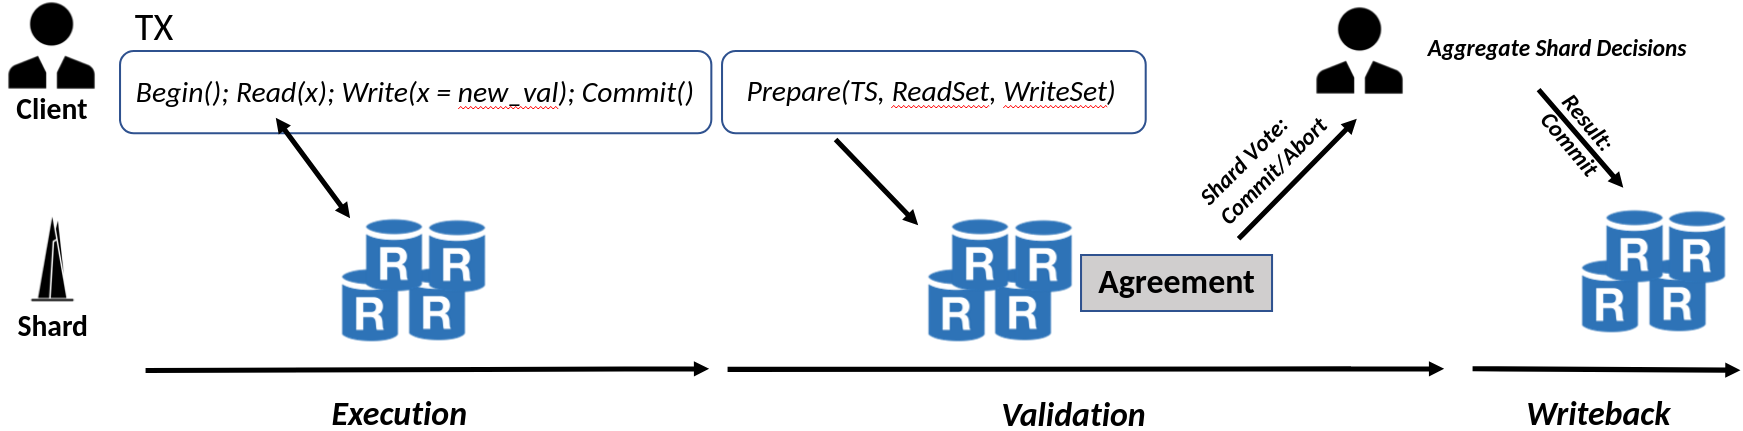
\includegraphics[width= \textwidth]{./figures/LC.png}
\end{center}
\caption{Transaction Lifecycle}
\label{fig:Figure1}
\end{figure*}




\subsection{System Model}

We adopt the standard adversarial assumptions of BFT replication. We assume that an arbitrary but finite number of \sys's client are faulty, and that, within each shard, the number of faulty replicas does not exceed a threshold \textit{f}. Faulty clients and replicas may deviate arbitrarily from their correct specification; a strong but static adversary can coordinate their actions but cannot break standard cryptographic primitivives
%\changebars{}{like collision-resistant hashes, encryption, and signatures. We denote a message $m$, signed by principal $p$ as $\langle m \rangle_p$}.

\sys{} does not rely on network synchrony for safety, though it is live only as long as messages exchanged between correct parties are delayed by no more than a fixed, but potentially unknown time interval~\cite{castro1999practical, fischer1985impossibility, kotla2007zyzzyva, clement2009making, buchman2016tendermint}.

We assume that clients are authenticated, and access control enforced: though these steps do not prevent  authenticated Byzantine clients from compromising the database's integrity, they enable auditing of their actions. 

%\sys{}  does not rely on network synchrony for safety; however, it can only guarantee liveness when messages exchanged between correct parties are delayed by no more that a fixed, but potentially unknown time interval~\cite{fischer1985impossibility}}.

% Further, \sys{] guarantees liveness one a per-client basis:
% Unlike traditional State Machine Replication protocols, where client liveness  in which the liveness of all Clients is correlated with the fate of the system (or often more specifically a leader), our system guarantees liveness not on a system basis, but on a per client basis. Concretely, we only guarantee liveness to clients that follow the protocol. Conversely, an honest client only loses liveness when it intertwines its fate with byzantine clients.\\

% The influence of Byzantine clients may be reduced by enforcing authentication and access control; though it is impossible to prevent authenticated Byzantine clients from compromising the database's integrity, their actions are  retraceable by auditing transaction logs 
\subsection{System properties}
%\fs{honest not yet defined.}
%\fs{is saying: byz can explicitly violate ACID semantics too strong?}
To express \sys's correctness guarantee, we introduce a general property we call  {\em Byzantine isolation}. Informally, Byzantine isolation offers to correct participants the view of an ACID compliant state, even in the presence of Byzantine actors;  while Byzantine clients may choose to explicitly violate ACID semantics, they cannot cause correct clients to observe an inconsistent state.  
%Indicus offers clients an interactive transaction interface that maintains the view of an ACID compliant state to all honest participants. Byzantine clients instead, may choose whether to experience isolation guarantees, but cannot tamper with "honest observable" state.
%Concretely, Indicus defines and implements \textit{byzantine Serializability}. Intuitively this Isolation level guarantees that all honest clients perceive the database as if were serializable. In order to formally capture this we lay some ground work: 
%\footnote{We modify and expand on definitions for BFT-linearizability from \cite{liskov2006tolerating}}


\nc{would like to emphasise that this is an independent contribution, and not linked to the system specifically}
More formally, we start from  the standard notions of transactions and histories introduced by Bernstein et al~\cite{bernstein1987concurrency}. A transaction \textit{T} executes read and write operations and either commits or aborts. A history \textit{H} is a partial order representing the interleaving of concurrently executing transactions, such that all conflicting operations are ordered with respect to one another. We additionally define \textit{C} to be the set of all correct ($Crct \subseteq K$) and Byzantine ($Byz \subseteq C$) clients in the system.
% A client is \textit{} if, given a protocol $P$, it follows $P$.
A projection $H|_{c}$ is the subsequence of requests in $H$ that were issued by client $c$. Drawing from the notions of BFT linearizability~\cite{liskov2006tolerating} and view serializability~\cite{bernstein1987concurrency}, we then define the following properties:

% \par\textbf{Honest History H(P)} Given protocol P, a \textit{history H} is \textit{honest} if it was generated by participants who all follow P, i.e: $H(P) \equiv H = H|_{Hon}$.

\par\textbf{Legitimate History (H$_L$)} History $H$ is \textit{legitimate} if it was generated by correct participants, i.e., $H_L \equiv H = H|_{Crct}$.

\par\textbf{Legit-View Equivalent} \fs{the name doesn't flow as much; honest-view better conveyed the intuition, i.e. all correct view it equivalent..} History $H$ is \textit{legit-view} equivalent to a history H' if all operation results, commit decisions and final database values in H's correct projection match those in H'.

%OLD: the operations and decisions of all honest clients are the same and if the final writes are the same.
%\nc{I have a question: the final writes here is a bit confusing because it sounds like we are requiring writes of byzantine clients to be the same here}
%\fs{added final state to NC updated version. Its only view equivalent if all read results are the same, and the database ends up in the same state.}

% \par \textbf{Byz-I} Given a protocol $P$ and an isolation level $I$:
% a history $H$ is \textit{byzantine-I} if there exists an honest history \textit{H'} such that H is honest-view equivalent to H' and H' satisfies I.

\par \textbf{Byz-I} Given  an isolation level $I$,
a history $H$ is \textit{Byz-I} if there exists a legitimate history \textit{H'} such that $H$ is legit-view equivalent to $H'$ and $H'$ satisfies $I$.

% This definition captures the requirements for any byzantine tolerant protocol that strives to maintain byzantine isolation level Byz-I. Informally, a byzantine Isolation level states that the state that honest clients experience must be explicable by an execution in which all participants were honest. Note, that we make no assumptions on the state a byzantine client chooses to experience; Byzantine client reads may be arbi- trary, i.e. read values need not respect I, nor correspond to writes that were ever written! Indicus maintains byzantine isolation level Byz-Serializability.

This definition is not \sys-specific, but captures the correctness requirement of any Byzantine-tolerant database that strives to maintain isolation $I$. Because it is  expressed in terms of properties of client-observable states, it is easier for applications to relate to both the guarantees it offers and the anomalies it allows~\cite{crooks17seeing}; informally, it requires the states observed by correct clients to be explicable by an execution that involves only correct participants.  Note that we make no assumptions on the states  Byzantine clients \textit{choose} to observe; the values they read may not respect $I$, or even not be the product of previous writes!


\nc{If we have a real estate, I would love for us to emphasise why this is cool, and how this is all based on the notion of equivalent to what clients actually observed .. client-centric.. view equivalence etc. It would also be kind of cool to show an example} \la{I tried to do a little of this by massaging the text.}

%
%Let $Op =  \{r, w\} \times K \times V $ and $Dec = \{Commit, \,Abort\}$ be the sets of possible read/write operations and decisions respectively, where $K$ is the set of existing data items (keys) and $V$ the range of possible values. A \textit{request} $req \in (Op \cup Dec) \times C$ maps any such operation or decision to the issuing Client from set $C$. We denote with $Hon \subseteq C$ the subset of honest Clients. 
%%\fs{could alternatively define ops as functions r[x] and w[x], and dec as c/a}

%\fs{NEW ALTERNATIVE: Def from \cite{bernstein1987concurrency}: (formal details commented in tex)}

%A \textbf{transaction T}, $T \coloneqq (REQ, <_T)$, consists of a set $REQ \coloneqq \{req_1, \dots, req_t \}$ of requests issued by some client $c$, and a partial order relation $<_T$ such that a) $REQ$ contains a finite number of operations, and exactly one decision $req_t = (dec \in Dec, c)$, b) $<_T$ induces a total order for every read and write operation on a shared key $k$. 
%%\fs{, either $(r, k, v_r) <_T (w, k, v_w)$ or $(w, k, v_w) <_T (r, k, v_r)$}, and c) all read/write operations precede the decision. 
%%\fs{for all read and write operations $(\{r,w\} \times k \times v) <_T dec$.}

%\textbf{History H.} A History represents the interleaving on concurrently executed transactions. Concretely, we define a \textit{history} $H \coloneqq (R, <)$ as partial order where $R$ and $<$ are supersets of a finite set of transactions, i.e. $R \supseteq \bigcup_i T_i$, and $< \supseteq \bigcup_i <_{T_i}$ .
%Let $Committed(H)$ be the subsequence of all Transactions with $req_{t} = Commit$. A History H is legal if every read request $(r, k, v)$ is preceeded by a matching write request $(w, k, v)$
%and there is no other write $(w, k, v')$ inbetween.
%% \fs{could formalize this: $\forall (r, k, v).\exists (w, k v). (w,k,v) < (r,k,v) \land \neg \exists (w, k, v'). v\neq v' \land (w, k,v) < (w,k, v') < (r, k, v)$}
%For two transactions $T_a$ and $T_b$, we denote $T_a < T_b$ iff $\forall req^a_i, req^b_j \in T_a, T_b. req^a_i < req^b_j$. A history is serial if all transactions are executed sequentially: $\forall T_a, T_b: T_a < T_b \lor T_b < T_a$.
%
%\textbf{Serializable} 
%A history H is serializable if there exists a serial permutation H' of Committed(H) such that H' is legal.
%
%
%\fs{Old TX def in comments. It is shorter... but lorenzo prefers the berstein def}

\iffalse
\textbf{History H.} We define a \textit{history H} as a finite sequence of requests. Informally, a \textit{H} contains the operations (read/write) and decisions (commit/abort) of every transaction issued in the system.

We define a projection $H|_c$ as the subsequence of requests in $H$ that were issued by Client $c$. A sequence of requests $s = req_i \dots req_{i+t}$ in $H|_c$ form a \textit{Transaction} if $req_i$ is the first request by Client $c$ or $req_{i-1} \in Dec \times c$, and if $req_{i+t} \in Dec \times c$. Let $Committed(H)$ be the subsequence of all Transactions with $req_{i+t} = Commit$. A History H is legal if every read request $(r, k, v)$ is preceded by a matching write request $(w, k, v)$ and there is no other write $(w, k, v')$ inbetween.\\
\textbf{Serializable}  
A history H is serializable if there exists a serial permutation H' of Committed(H) such that H' is legal.
\fi
%
%We define a projection $H|_c$ as the subsequence of requests in $H$ that were issued by Client $c$.
%We further define:\\
%\textbf{Honest History H(P).} Given protocol P, A \textit{history H} is \textit{honest} if it was generated by participants who all follow P, i.e: $H(P) \equiv H = H|_{Hon}$.\\
%\textbf{Honest-View Equivalent.} A \textit{history H} is honest-view equivalent to a \textit{history H'} if the Operations and Decisions of all honest Clients are the same and if the final writes are the same.\\
%\textbf{Byz-I} Given a protocol $P$ and an isolation level $I$:
%A history H is \textit{byzantine-I} if there exists an honest history \textit{H'} such that H is honest-view equivalent to H' and H' satisfies I. \\
%
%This definition captures the requirements for any byzantine tolerant protocol that strives to maintain byzantine Isolation level I.
%Informally, a byzantine Isolation level states that the state that honest clients experience must be explicable by an execution in which all participants were honest. Note, that we make no assumptions on the state a byzantine client \textit{chooses} to experience; Byzantine client reads may be arbitrary, i.e. integrity \fs{based on real commit} and legality \fs{based on latest write} of both read values and versions need not be maintained. Indicus maintains byzantine Isolation level Byz-Serializability.\\
%
%\fs{cut the next part about byzantine Atomicity: Need to mention somewhere that only writes experience atomicity. Reads from byz clients are not required to be included}
%\fs{Look at tex comments.}
%\iffalse
%We further define \textit{byzantine Atomicity}. Intuitively, only honest client transactions are guaranteed to experience Atomicity, i.e. all of its operations succeed, or fail jointly. It follows straightforward:\\
%\textbf{Byz-A} Given a protocol $P$, a history $H$ and a set of honest client $Hon$. All \textit{Transactions} in $H|_{Hon}$ experience Atomicity, i.e. either all requests are committed, or not a single request is committed.\\
%\fs{This may not be ok if validation maintains Invariants based on the assumption that a Tx is atomic or not: I.e. a bank transfer is net 0. In this case we need to enforce atomicity on writes - cannot on reads since they may not be included - replicas must include all shards for its writes (currently i made it optional so that shards reject it themselves- this makes shards oblivious to what items are in other shards).}
%
%Indicus maintains both \textit{Byz-I} for Isolation level Serializable and \textit{Byz-A}. 
%In more pragmatic terms, all honest clients experience the ACID properties, whereas byzantine clients may \textbf{choose} whether to experience Atomicity and Isolation for their transactions.
%\fi
%

Specifically, \sys{} guarantees Byz-Serializability.  This is a strong safety guarantee, but it does not enforce application progress; a Byzantine serializable system could still allow Byzantine actors to systematically abort all transactions. To preclude such pathologies, we explicitly define the notion of \textit{Byzantine independence}, a %progress \la{ this seems to me to be a safety property!} 
system property that bounds the influence of Byzantine participants on the outcomes of correct clients' requests.
%Next, we define an ideal progress property to limit the influence byzantine participants have on honest clients.
%\fs{Byz Indep is the liveness property, whereas Byz Serializability is the safety property. Without Byz Indep any protocol could be trivially Byz serial by just aborting all. }

% \par \textbf{Byzantine Independence} The result of a request $r$ issued by a correct client $c$ cannot be deterministically decided by Byzantine participants. %\fs{in 5f+1 we can strengthen this to hold for byz client c too.}



 \par \textbf{Byzantine Independence} For every request $r$ issued by a correct client $c$, there exists no group of participants that can dictate the result of $r$, and contains only byzantine actors.

\fs{perhaps it currently sounds too strong, I am not sure whether the "reliably" part is captured.}
\fs{explicitly phased as request and not transaction, so it is applicable to general SMR. For us: applies to reads: therefore we want to read from f+1, applies to transaction outcome: therefore we dont want a leader. If the adversary controls the network, then a single byz client can be that group. (applies to both reads and tx commit/abort). If you want to read from a single replica, then you are explicitly giving up byz independence for that request}

  
  
  
\iffalse  
\par \textbf{Byzantine Independence}  The result of a request $r$ issued by a correct client $c$ cannot be deterministically decided by Byzantine participants. %\fs{in 5f+1 we can strengthen this to hold for byz client c too.}
\la{Should it be expressed in terms of requests or transactions? If so, the next sentence is unnecessary. More importantly, I don't know what ``deterministically decided'' means. There would have to be somewhere a universal quantifier (``for all executions'') but it is not clear what is the set of events over which we consider all possible executions.}
 \fi

Byzantine independence implies, for instance, that Byzantine actors cannot collude to singlehandedly abort an honest client's transaction. \nc{I think an example would be great here}. This is a challenging property to enforce. %In leader-based systems, for example, by colluding with Byzantine clients a Byzantine leader may 
\la{I am weary of the ``always'' without a proof. By the way, there must be something we are assuming about what is necessary for a leader to inject conflicting operations--it seems, for instance, that it would at least require some collusion with a Byzantine client: a proof would allow us to create a propoerly qualified statement}
In fact, no leader-based system can guarantee Byzantine independence: a Byzantine leader may always inject conflicting operations that cause transactions to abort
\nc{we could use this example in a picture?}. Without additional network assumptions,
\sys{} also cannot enforce this property: for \sys{} to enforce Byzantine independence,a global adversary cannot have global control over the network (and thus fully determine message arrival order). We note that even with this stronger model, Byzantine independence is still unattainable for leader-based systems.

%
%\changebars{}{Intuitively, byzantine independence implies, that honest clients' transactions cannot be reliably, strategically aborted by byzantine influence. If the network is controlled by an adversary, this property is unattainable for Indicus.
%%\footnote{We point out, that all leader-based protocols suffer the same fallacy: A byzantine leader may always frontrun/inject requests that influence successive transaction results. In fact, even with strengthened network assumptions, such a a system could not offer Byzantine Independence. }}
%In order to offer this property we must strengthen our assumption on the network. Concretely, while the network may be asynchronous, we assume the adversary does not control the network, and hence, may not reliably impact results \footnote{An exception to this are wide-ranged flooding attacks (ddos) which are beyond the scope of this work.}. \fs{Not only can byz not influence results, but they cannot perform front-running - i.e. submit tx at earlier time based on knowledge of later tx. Maybe this distinction needs to be clearer in the definition}
%
\iffalse
\fs{omit this next part. gracious potentially useful to talk about Fast Path. Uncivil not really}
We adapt and define gracious and uncivil executions based on cite(aardvark) to match our model. (i.e. network not sync either).
\textbf{Gracious Execution}
An execution is gracious iff (a) the execution is synchronous with some
implementation-dependent short bound on message delay (b) all clients and servers behave correctly and (c) there is no contention on the objects relevant to the execution.
\textbf{Uncivil}
An execution is uncivil iff (a) there is no bound on message delay (asynchrony) and (b) up to f servers and an arbitrary number of clients are Byzantine 
\fi



\subsection{Discussion}
\nc{I wasn't sure what to do with this paragraph. On the one hand I like it,
on the other it's not obvious to me that it's necessary. What I do think
is that the part on clients in the client model should go here. I attempted a much 
shorter version but I'm not sure that this is better. It completely removes the "reactive" behaviour, which i understand is cool, but i'm not sure people will appreciate this. I think it acts better as a transition paragraph into the rest of the sections}

The literature offers two main approaches to dealing with Byzantine bahaviors: \one~ BFT systems attempt to mask Byzantine actors, and thus strive to guarantee both safety and liveness in their presence; \two~ systems that provide  accountability do not provide safety, but discourage Byzantine actors by guaranteeing they will eventually be linked to their actions.  \sys{} leverages its system model to take a hybrid approach. On the one hand, it uses BFT to guarantee safety in the presence of Byzantine  behavior; on the other, being a permissioned system, it uses tamper-proof transaction logs to disincentivize  Byzantine behaviors that undermine the system's liveness.  Thus, \sys{}'s design leans towards  being efficient during fault-free executions; when misbehaviour does occur, \sys{} remains safe while bounding overheads, using auditing to address sustained attacks to its liveness.  We achieve this balance through the design of aggressive concurrency control mechanisms, which we combine with recovery protocols that enforce independent operability.

\fs{NC version in comments}

% While \sys{} remains safe under byzantine attacks, we do not expect that these will be frequent in practice. Clients are incentivised to maintain standing in a permissioned system, and thus unlikely to engage in actively detectable byzantine behaviour, as this would result in them being removed from the database~\cite{drushel's work}. To this effect, we design \sys{} to minimise costs during gracious executions while bounding overheads when misbehaviour does occur. We achieve this balance through the design of aggressive concurrency control mechanisms, which we combine with recovery protocols that enforce independent operability.


\fs{old FS version with reactive behavior in comments. I think its good to mention that clients would need access control and network in order to do targeted artificial congestion. }
\iffalse
While we allow clients to act arbitrarily and maintain safety unconditionally, in practice, we do not expect clients to intentfully attempt to circumvent other clients progress via targeted congestion. We deem this assumption reasonable as a byzantine client requires both prior knowledge on  honest clients' transaction patterns as well as relevant access control in order to artificially increase object contention. In Indicus, we assume network neutrality in order to defend against explicit \textit{reactive} artificial contention and maintain Byzantine Independence.
We assume that actively detectable byzantine behavior (such as equivocation or other protocol incoherence) is rare as clients are incentivised to maintain standing in a permissioned system.
Moreover, we exect an appropriate level of client performance, from both honest and byzantine clients, to qualify for system participation. Untimely behavior may qualify as misbehavior and elicit client expulsion. 
\fi

%%%
\iffalse
\fs{Replicas can enforce client expulsion via access lists, i.e. via timeouts of blacklists. A strawman protocol to agree on client expulsion can look as follows: 1) If a replica has a PoM (i.e. a equivocation proof, false abort without cert) it may forward this evidence and ignore the client immediately. 2) If a client frequently times out on a client (i.e. either its read timestmap expires - we discuss lighter penalties in section Personalized Read Leases - or a fallback election is started) a replica submits a vote of untimeliness by broadcasting to all replicas. Upon reception of 2f+1 votes (this implies that there might be no progress) a replica blacklists the client and forwards the vote, guaranteeing that every correct replica will do the same. (Alternatively we could forward once f+1 are received, but only blacklist when 2f+1 are received. But this means that the client could have been making progress overall, so it is overly conservative). A honest replica may remove all tentative client associated transaction state upon blacklisting, as it is guaranteed that all other honest replicas will do the same. Waiting dependencies must be aborted.}


Given these client expectancies, we design Indicus to minimize costs during gracious execution while defending and bounding the overhead accordingly when misbehavior does occur.
\fi




%-------------------------------------------------------------------------------
\subsection{Execution}
%-------------------------------------------------------------------------------
- Read proofs required for honest client correctness. Alternatively one can read from f+1 only, but that can result in failed/older reads
- Do not need to include read proofs in the prepare. According to Isolation definition byzantine Clients can read whatever they want. Moreover, Reads only have very limited external effect. The value does not matter for the CC check. The version has bounded effect: If it goes towards 0, then it is just a check between timestamps as normally. If it goes towards the TS, then it will never abort.
- Fallback not just useful for dependency cleanup, but also "unclaimable" dependencies that need to finish.
%-------------------------------------------------------------------------------
\subsection{Validation}
%-------------------------------------------------------------------------------

%-------------------------------------------------------------------------------
\subsection{Concurrency Control}
%-------------------------------------------------------------------------------
 - Optimization: retries - heights
 - Dependency resolution tree
 		- Equivocation not possible if TXidentifier a function with dep as argument
 		- Cannot claim dep if not f+1 times (If you want to, you would require proofs again, which we try to avoid because dep trees can grow exponentially). More reads also more likely to commit --> f+1 guarantees 1 honest thinks it is legit.
 - Exception for depedency and early async read response to inform of exceptions
 - Read leases instead of unlimited locks - in practice only grant to timely clients (not a safety measure, but an increased progress guarantee)
 - 
%-------------------------------------------------------------------------------
\subsection{Consistent logging.}
%-------------------------------------------------------------------------------
Principles and challenges

protocol overview: pic


%-------------------------------------------------------------------------------
\subsection{Writeback and Multi-shard 2pc}
%-------------------------------------------------------------------------------

- Optimization: Single shard logging
%-------------------------------------------------------------------------------
\subsection{Failures}
%-------------------------------------------------------------------------------
- Fallback: election (only starts if not waiting on another dep to avoid early eviction), views, resolution, subtelties with mvtso (block because of dep), necessity even without dependencies. Interested clients, write-back multishard. garbage collection
- Fallback requires an extra round in order to learn about current views to start viewchange, but thats ok: Its co-function with learning about full TX, and checking for existing certificates. Timeout invocation is concurrent with p1 message.

%-------------------------------------------------------------------------------
\subsection{Low Cost mode}
%-------------------------------------------------------------------------------
3f+1 if not defending against byz colluders
OCC if not worried about reads aborting


%-------------------------------------------------------------------------------
\section{Implementation and Evaluation}
%-------------------------------------------------------------------------------


%-------------------------------------------------------------------------------
\section{Limitations}
%-------------------------------------------------------------------------------
Shifting responsibilites from replicas to clients comes at the cost of higher computational requirements for clients which may not be tolerable for some applications that demand lightweight clients \cite{gueta2018sbft}. In practice, we envision \sys clients to be dedicated transaction managers, that provide an interface for light-weight end-users. 

As is inherent to any system leveraging optimistic concurrency control, \sys is vulnerable to highly congested workloads and must yield the abort of some transactions to maintain isolation guarantees. Note however, that when clients conduct transaction execution, a pessimistic, locking-based concurrency control (i.e. 2PL) incurs deadlock resolution on the same order of frequency, yet requires additional coordination overhead. Speculative execution however, is inherent to an interactive interface; applications striving for deterministic committability must restrict their transaction model and/or rely on serial execution (i.e. SMR). 

Similarly, as is the case for most BFT protocol, \sys is vulnerable to ddos attacks by byzantine participants. A byzantine client with unrestricted access control may subverting progress for honest users by artificially increase congestion. Defense against fllod-based attacks is out of scope of our work, but is disincentivised as participants are accountable in permissioned membership groups. We remark that clients in \sys can deterministically abort transactions (byzantine independence) only when controlling the network.



\iffalse

Shifting responsibilites from replicas to clients comes at the cost of higher computational requirements for clients. This may not be tolerable for some applications, and other existing systems (i.e cite sbft) structure their design explicitly to be compatible with lightweight clients. In practice, we envision Indicus clients to be dedicated transaction managers, that provide an interface for light-weight end-users. For example, in a distributed stock market, brokers may act as transaction managers in lieu of their clients.

As is inherent to any Optimistic Execution and Concurrency Control, Indicus is vulnerable to highly congested workloads. When contention on select objects is high, concurrent execution of Transactions must yield the abort of some Transactions during Validation in order to maintain the Database Isolation guarantees. 
\fs{When contention is very high, it can be desirable to in fact have a total order. Doing just validation in total order wont reduce aborts though. Requires transactions to be pre-defined }

Note however, that when clients are in charge of execution, a pessimistic concurrency control solution such as two-phase-locking would incur an equal amount of deadlocks which would require resolution. The observation to make is that any system that conducts execution at the client application side speculates on concurrency. This however we stipulate, is unavoidable when trying to scale a system to the number of users rather than replica processing power. The traditonal ways to avoid the abort rate conundrum is to either restrict the transaction model, which in turn weakens the general applicability of the protocol, or to delegate execution to replicas and utilize State Machine Replication to serialize Transactions. SMR protocols with a single leader do not inquire any congestion based aborts as a single sequencer naturally eliminates concurrency.
Indicus does not make these concessions in order to offer interactive Transactions and remain scalable. A workload that exhibits low commutativity and high contention should therefore refrain from adopting our system.

Similarly, as is the case in any transaction protocol, Indicus is vulnerable to ddos attacks by byzantine participants. A byzantine clients only opportunity at subverting progress for honest users is to artificially increase congestion. When such a client has unrestricted access control it may do so strategically iff it has control over the network. If it does not, it cannot reliably gain knowledge about concurrent transactions before they pass the validation step and must resort to flooding based attacks. Defense against such attacks is out of scope in our work, but is disincentivised as participants can be held accountable for their actions in a closed membership setting.


\fs{technical limitations: We require more replicas to avoid certificate signature overheads. Since in 3f+1 one decision needs to be enough to recover. byzantine replicas/clients have more power to vote arbitrarily, because they cannot be held accountable for it. In total order protocols (SMR), deviation from the "common" vote signals misbehavior, whereas for us that is not the case. --> this should go as a challenge somewhere.}

\fs{Clients are more heavyweight. Not suitable for settings where clients just have minimal processing capacity. In practice we envision clients to be dedicated transaction maangers.
Also, Clients need to be registered in system with a sig - necessary to enforce access control in any system however}
\fi


%-------------------------------------------------------------------------------
\section{Related Work}  
%-------------------------------------------------------------------------------

\paragraph{Consistent Replication}
Indicus offers a replicated, byzantine fault tolerant database that leverages concurrency control and quorum based agreement to maintain isolation guarantees despite its unordered/inconsistent replication layer. 
The majority of prior work instead maintains consistent replication by means of the State Machine Replication (SMR) approach \cite{schneider1990implementing}. Existing replication solutions for the crash failure fault model (Paxos based: \cite{Li2007, Lampson2001, Lamport98Paxos, Lamport2005a, Lamport2005, Lamport01Paxos, Chandra2007} , Zab: \cite{junqueira2011zab}, \cite{van2014vive}  VR: \cite{oki1988viewstampeda, liskov2012viewstamped}, Raft: \cite{ongaro2014search}) as well as the byzantine fault model \cite{lamport2011byzantizing, pires2018generalized, Guerraoui08Next, Kotla04High, bessani2014state, liskov2010viewstamped} (most notably PBFT \cite{castro1999practical}) maintain consistency by achieving consensus on a totally ordered log of requests. They are, in addition, primarily leader-based which introduces additional scalability issues~\cite{epaxos,tapir} as well as fairness concerns. Recent efforts to address this bottleneck can be classified in three ways. Then you have your enforcing PO, fine-grained ordering, sharding}

The seminal \textit{practical} Byzantine Fault Tolerance (PBFT) protocol and its adaptations (cite Zyzzyva, aardvark..) form the cornerstone of most Permissioned Blockchains \cite{Hyperledger, EthereumQuorum, buchman2016tendermint, al2017chainspace, kokoris2018omniledger,  gilad2017algorand, baudet2019state} (Algorand and Omniledger both not permissioned, but lots of PoS blockchains elect validator set that runs pbft basically, mention some traditional blockchains? Bitcoibn, Ehtereum, also total order).

\fs{mention zyzzyva explicitly because of Fast path concept and speculative execution of replicas. Difference: still leaderbased and clients EXPECT replicas to process in order.}


\paragraph{Enforcing Partial Order}
Totally ordered ledgers solve the problem of consistent transaction replication but enforce unecessary coordination/serialization between commutative operations. 
Approaches to reconcile this scalability limitation by inducing only a partial order can be broadly categorized in three ways:
\textbf{1. Fine-grained ordering}: One class of approaches attempts to only order conflicting operations by leveraging transaction semantics. Existing work however (cite all CF: Epaxos, Generalized Paxos, \cite{sutra2011fast}, \cite{li2012redblue}, Curp, Carousel, MDCC, Tapir, Janus) targets almost exlusively the crash failure model. To the best of our knowledge, Bilbos/Clairvoyant is the only BFT system that offers SMR for commutative transactions, but unlike Indicus is limited to a static transaction model and introduces blocking, as any transaction must wait for all potentially concurrent transactions to complete. Other quorum based systems whose strucutre Indicus resembles (Q/U, H/Q, Liskov rendering harmless) allow for commutativity, but do not offer transactions. \fs{Q/U resembles Logging in Indicus - but has no liveness on its own.}

\textbf{2. Sharding} In the blockchain space, sharding has been explored as mechanism to parallelize independent transactions across shards, while relying on total-order primitives within (Omniledger, Chainspace); In Indicus we argue however, that inducing a partial order via sharding is merely a limited engineering optimization. Existing work in the crash failure model (Tapir, Ordering Paper, Janus) points out that layering sharding and transactional control on top of replication (cite Spanner?) incurs redundant coordination, and improves performance by integrating both layers. Indicus is the first to adopt this rationale in the byzantine fault model.

\textbf{3. DAGs} Lastly, the use of Directed Acyclic Graphs (DAGs) that allow to parallelize agreement instances, has been explored in several permissionless blockchain networks (Iota, Byteball, Ava, overview paper). It remains unclear whether practical applications exist for the permissioned setting - designing a BFT protocol that replicates a DAG instead of a totally ordered ledger is an interesting avenue for future work.


\paragraph{Byzantine Databases}
In Indicus we argue that blockchain functionality, i.e. a distributed transactional system, should be captured by a BFT Database (DB). There exist a series of work offering explicit BFT DBs  
cite( Byzantium, Augustus, Callinicios, HRDB, BFT Dur, Databasify Fabric): HRDB offers interactive transactions for a replicated DB, but relies on a trusted shepherd layer. Byzantium designs a middleware system that utilizes PBFT as atomic broadcast (AB) and provides Snapshot Isolation via a primary backup validation scheme. In cite(BFT Dur) Pedone et al. too, rely on AB to design an OCC-architecture similar to Indicus. Augustus and Callinicos leverage sharding for scalability by assuming a limited comparison/query/update transaction model and implementing an optimistic and locking based execution model respectively on top of atomic broadcast.
We expand on existing research to 1) be leaderless and more scalable by allowing un-ordered replication rather than AB, 2) provide interactive transactions, and 3) offer sharding for horizontal scaling.
\subparagraph{Byzantine Clients}
Existing work concerned with byzantine clients addresses mechanisms to reduce frequency and severity of client misbehavior (BFT-dur, byzantium, agustus, callinicos, others, byz liskov). We reformulate transactional corectness guarantees in a byzantine setting to be more explicit about byzantine client behavior \fs{too vague} and extend Liskov et al.s (cite rendering byz client harmless) definition of Byz-Linearizability to transactions (Byz-Serializability). 
Lastly, Herlihy (cite) discusses mechanisms to improve fairness in leader-based systems - In Indicus we sidestep fairness concerns by being leaderless and instead define Byzantine Independence in order to formalize byzantine influence.











\subsection{details}


Indicus is the first to do blablabla. This section describes related work...

\textbf{Distributed Transactions for benign faults}
A lot of recent effort has gone into designing high throughput and low latency databases that leverage synergies between transaction and replication layer to improve performance. The recently proposed TAPIR transaction protocol leverages redundancy between transaction ordering and replication ordering to reduce total roundtrips, thus reducing latency in wide area networks. TAPIR shares several similarities with our system, most notably the absence of a leader and the resulting unordered validation structure. Like Indicus, TAPIR utilizes optimistic concurrency control to allow for concurrency among commutative transactions while minimizing coordination. When congestion is high however, throughput and tail latency worsen as abort rate grows. Janus avoids transaction aborts by dynamically re-ordering conflicting transactions \cite{mu2016consolidating}. This however, is made possible by assuming one-shot transactions, i.e. fixed read/write keys, and thus reduces the application generality. Another key-value store, Carousel, similarly assumes a restricted Transaction model in order to parallelize execution and validation \cite{yan2018carousel}. CURP too, leverages commutativity in order to reduces replication costs by making requests durable first, and only ordering them later \cite{park2019exploiting}. 

While all of these databases offer low latency replication, they are fundamentally limited to tolerating crash-failures. This strong failure assumption makes them less robust and not suitable for mission-critical services \cite{Abdollah2007}, finance or otherwise highly sensitive data.

\textbf{Byzantine Fault Tolerant Replication} 
\fs{Really not necessary to explain all the different SMR protocols that exists. Rather: Should explain how they could be used to solve the same problem with total order?}
 The problem of tolerating arbitrary failures was originally formalized as \textit{Byzantine Generals Problem} \cite{lamport2019byzantine}, paving the way for countless Byzantine Fault Tolerant (BFT) protocols and implementations \cite{castro1999practical, martin2006fast, kotla2007zyzzyva, pires2018generalized, bessani2014state, lamport2011byzantizing, arun2019ezbft, malkhi2019flexible, duan2014hbft, yin2003separating}. Such protocols have a reputation of being  both notoriously difficult to understand and design correctly \cite{abraham2017revisiting, abraham2018revisiting, shrestha2019revisiting}, and in practice often impose significant overhead compared to its crash-failure tolerant counterparts, hence limiting frequent industrial adoption.
Recently however, with the surge in Blockchain interest, BFT protocols are experiencing a second Spring. While originally developed to tolerate arbitrary bugs, these protocols find increasing importance in settings where participants are untrusted or malicious. Permissioned Blockchains, organized by a consortium of registered participants can use traditional BFT State Machine Replication (SMR) protocols in order to achieve agreement. 
\fs{mention basic BFT first? pBFT is the first "practical", not the first BFT}
The seminal practical BFT (PBFT) protocol \cite{castro1999practical} implements a primary backup scheme that achieves consensus in three broadcast rounds, maintaining safety as long as the number of faulty participants is $<1/3$ (i.e. $n\geq 3f+1$), and offering liveness during synchronous operation. When primaries misbehave, a dedicated \textit{view-change protocol} allows for safe reconciliation. There have been numerous adaptations that aim to speed up common case and failure free execution such as FaB \cite{martin2006fast}, and most notably Zyzzyva \cite{kotla2007zyzzyva} which leverages speculative execution and a semi-client driven protocol to reduce latency. Akin to Indicus, replicas in Zyzzyva speculatively execute requests out-of-order, and rely on honest clients for reconciliation. Zyzzyva replicas however, \textit{expect} to process requests in-order, and diverge only temporarily as result of a byzantine leader. hBFT builds on Zyzzyva and attempts to improve faulty case behavior by returning the client responsibility of detecting inconsistencies to a dedicated replica checkpointing protocol. 
UpRight explores efforts to tolerate both byzantine and crash failures in order to make the overhead of deplyoing a BFT system practical.
SBFT \cite{gueta2018sbft} pursues the goal of scaling to scale to large replication degrees, while offering light clients and high throughput under benign faults. It adopts the UpRight replication model, and modifies PBFT by utilizing collectors, threshold signatures and a fast path akin to Zyzzyva. 
Aardvark \cite{clement2009making} emphasizes the importance of robust performance under byzantine failures by adding increased client and replica checks and imposing frequent leader rotation by steadily increasing throughput requirements. Tendermint \cite{buchman2016tendermint} pushes this idea to the extreme by rotating leaders continuously, at the cost of assuming a synchronous network. Herlihy and Mor attempt to rigorize fairness properties for permissioned Blockchains and propose techniques to increase accountability for Tendermint specifically \cite{herlihy2016enhancing}.

HotStuff too, explores the use of rotating leaders by exploiting the symmetry in PBFTs phases in order to pipeline transaction processing \cite{yin2019hotstuff}. 
Nevertheless, all protocols derived from the PBFT family suffer from the leader bottleneck as well as enforcing a total order even on commutative operations. BFT-Mir \cite{stathakopoulou2019mir} identifies the proposal speed of a single leader as the practical bottleneck in most implementations and improves upon this by allowing all replicas to act as proposers.
Biblos \cite{bazzi2018clairvoyant} achieves leaderless SMR by leveraging a non-skipping timestamp protocol. It furthermore allows for commutative transactions to be executed in parallel at the cost of requiring read/write key sets to be known in advance. In order to preserve liveness however, Bilbos falls back to a PBFT resolution. \fs{Uses all to all, predefined TX, pbft fallback, timestamp phase and proofs required}
The Quorum/Update (Q/U) protocol too, offers leaderless agreement by leveraging Qurorums for a agreement in a limited read/write interface, but fails to terminate under contention \cite{abd2005fault}. To reconcile this shortocming, the Hybrid Quorum protocol (HQ) explores a hybrid solution, extending upon Q/U by adding a PBFT fallback path under contention \cite{cowling2006hq}. In \cite{liskov2006tolerating}, Liskov et Al explore improved byzantine Quorum protocols for a single Read/Write interface, giving special attention to bounding the effects of byzantine clients. 
\fs{BFT protocols under fire: \cite{singh2008bft} that one-size-fits-all protocols may be hard if not impossible to design in practice}
All of the above systems, including Indicus, guarantee Liveness only under the assumption of some degree of synchrony. This is consistent with the well known FLP impossibility result stating that no deterministic consensus solution may exist in the presence of asynchrony \cite{fischer1985impossibility}. Protocols such as Ben-Or's algorithm \cite{ben1983another}, HoneybadgerBFT \cite{miller2016honey} or BEAT \cite{duan2018beat} sidestep this result by introducing randomization, thus enabling probabilistic agreement even during asynchrony.

\textbf{BFT distributed transactions}
While the literature on BFT state machine replication is extensive, the efforts to offer a transactional interface for BFT are scarce. SMR itself can be utilized as a straw-man system to implement pre-defined Transactions (one-shot or stored procedures) by enforcing a common total order in which replicas will execute the transactions. \fs{Byz agreement apps for DB \cite{garcia1986applications}}
HRDB offers a dedicated BFT Database, but assumes a trusted shepheard layer, thus not being truly BF resilient \cite{vandiver2007tolerating}.
Byantium \fs{middleware stuff} offers Snapshot Isolation for Transactions by re-purposing PBFT as atomic broadcast. It executes requests only at a primary and uses replicas to validate results in the total order defined by the SMR protocol \cite{garcia2011efficient}. Augustus implements short-transactions, a limited, comparison/query/update transaction model that declares all operations before execution \cite{padilha2013augustus}. It offers scalability via partitioning and achieves consistency within partitions by utilizing atomic broadcast. While Augustus assumes an optimistic execution model that allows for aborts under concurrency, its follow up work Callinicos implements a locking scheme in order to avoid Transaction aborts \cite{padilha2016callinicos}. To do so efficiently it resorts to a limited transaction model that requires knowledge of read/write sets and otherwise locks an entire partition in order to guarantee mutual exclusion, thus voiding any concurrency. BFT Deferred Update Replication adopts an interactive OCC transaction model comparable to ours, allowing execution to be speculative at clients \cite{pedone2012byzantine}. However, it uses PBFT as atomic broadcast implementation to enforce SMR on validation, thus resorting to both a leader, and a total order on all requests. It moreover does not extend to multiple shards.

\textbf{Blockchains and Sharding}
In the Blockchain world, Chainspace \cite{al2017chainspace} and Omniledger \cite{kokoris2018omniledger} implement sharding by layering 2PC and atomic broadcast (within shards) for the UTXO transaction model. Rapidchain \cite{zamani2018rapidchain} offers efficient sharding for a permissionless system (what else? didnt read much, not so relevant). Hyperledger provides an enterprise-ready permissioned blockchain solution that simulates optimistic transaction processing by letting replicas speculatively execute Smart Contracts. While Hyperledger \cite{Hyperledger} describes itself as a shared database, it relies on a dedicated SMR ordering service that enforces a total order, and, in practice, only tolerates crash failures (Hyperledger uses Raft \cite{ongaro2014search}, a consensus protocol for the Crash-Failure model,  but can be extended to use PBFT). Sharma et al. attempt to \textit{databaseify} Hyperledger by adding database techniques such as transaction re-ordering in order to reduce aborts, but fundamentally maintains the totally ordered (Hyper-) ledger design \cite{sharma2018databasify}. \fs{Databasify paper: tries to add some bandaid db techniques to hyperledger. Transaction re-ordering (still total order), and early aborts.} 
 \fs{(Mention other Permissioned Blockchain systems: Ethereum Quorum? (uses Raft or IstanbulBFT = implementation of pbft)}

Directed Acylcic Graph (DAG) based consensus architectures \cite{pervez2018comparative}(IoT-chain, IOTA, Byteball - all are blockless) have been explored  in order to parallelize agreement and execution instances. While these approaches increase throughput by inducing a partial order, they target permissionelss settings (based on Proof of Work/Stake), rather than permissioned BFT-based solutions. To the best of our knowledge there exists no such system to this date, and it is unclear how to merge these approaches. Designing a BFT protocol that replicates a DAG instead of a totally ordered ledger is an interesting avenue for future work.






\fs{How does all this related work compare to Indicus?}



%-------------------------------------------------------------------------------
\section{Conclusion}
\label{section:conc}
%-------------------------------------------------------------------------------

summary of Indicus

Our experience designing Indicus.

opportunities for future systems? what kind of systems maintain the defs?

%-------------------------------------------------------------------------------
\section*{Acknowledgments}
%-------------------------------------------------------------------------------

The USENIX latex style is old and very tired, which is why
there's no \textbackslash{}acks command for you to use when
acknowledging. Sorry.

%-------------------------------------------------------------------------------
\section*{Availability}
%-------------------------------------------------------------------------------

USENIX program committees give extra points to submissions that are
backed by artifacts that are publicly available. If you made your code
or data available, it's worth mentioning this fact in a dedicated
section.

%-------------------------------------------------------------------------------
\bibliographystyle{plain}
\bibliography{ref}


%%%%%%%%%%%%%%%%%%%%%%%%%%%%%%%%%%%%%%%%%%%%%%%%%%%%%%%%%%%%%%%%%%%%%%%%%%%%%%%%
\end{document}
%%%%%%%%%%%%%%%%%%%%%%%%%%%%%%%%%%%%%%%%%%%%%%%%%%%%%%%%%%%%%%%%%%%%%%%%%%%%%%%%

%%  LocalWords:  endnotes includegraphics fread ptr nobj noindent
%%  LocalWords:  pdflatex acks